% Template PNSAC newsletter - Article
% Language: Latex
%

% Head

\title{Notes from the President}
\author{Richard Lodge}

\maketitle

Canada Day is now behind us.  We had an excellent day with a good
number of our volunteers showing off the North Star to the general
public. Judging by the activity around the plane all the day, we have
now developed a display format which is interesting to visitors.
Canada Day was the only day this year when the plane was on display to
the general public.

\begin{figure}[htbp]
   \vspace{2em}
   \centering
   %name of the graphic, without the path AND in EPS format:
   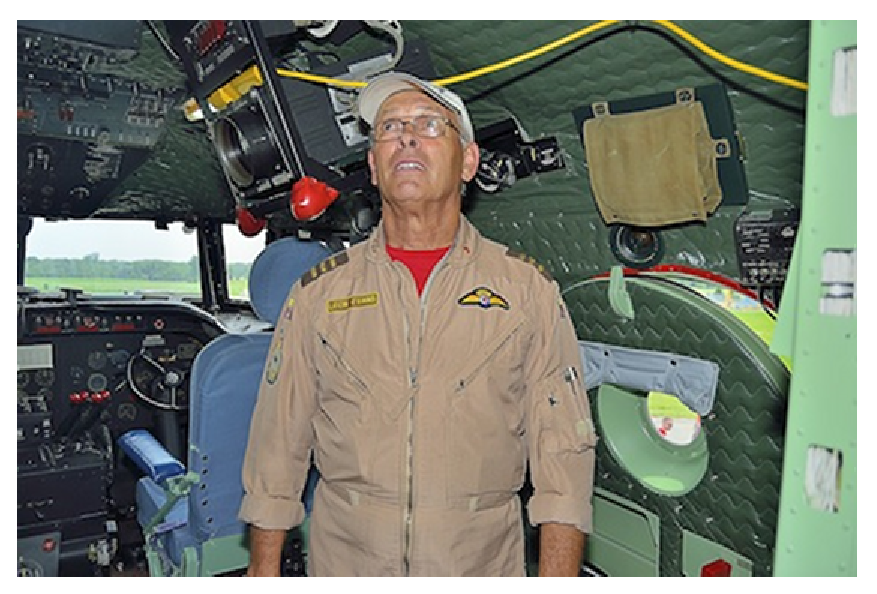
\includegraphics[scale=0.5]{canadaday_visitor.eps}
   %caption of the figure 
   \caption*{\small \em Showing off the North Star on Canada Day -- an
   impressed visitor examines the cockpit.}
   %label of the figure, which has to correspond to \ref{}:
   \label{fig:canadaday}
\end{figure}

On June 27, in co-operation with the Museum, who hosted the event, we
showed off the plane to a group of donors attending the Donor
Appreciation Evening.  This was a successful evening which is likely
to be repeated.

In my last Notes from the President, I referred to plans for
celebrating the 10th anniversary of the founding of the Project North
Star Association.  This should have taken place around June 24.
Unfortunately, the event passed without us being able mark the
day. This was mainly due to situations beyond our control.

Our 2013 AGM was held on June 8, and all the existing directors were
re-elected.  This will enable the directors, who have now become
experienced, to concentrate on long-term matters.

The actual work on the restoration of the plane is going very well, as
reported elsewhere in this newsletter. The major issue facing the
Board in the next year will be to consider how to secure the future of
PNSAC, both in terms of volunteers and the funding of restoration
work.

We have now reached a point where it is necessary to update our
Memorandum of Understanding (MOU) with the Museum and our work plan
for completing the restoration of the plane.  Our volunteers have
already worked over 60,000 hours on the project and we expect to work
a similar number of hours before the restoration is completed.

There have been several informal meetings to discuss our future
operations and the opportunities available for new volunteers.  Within
the next few weeks we are expecting to meet with the Director General
of the Aviation Museum and members of his staff to work on the MOU
update.

Later this month we are meeting with senior management of the Museum
Foundation, the body charged with corporate fundraising for the Canada
Science and Technology Museums Corporation, to discuss how PNSAC can
work with the Foundation to raise funds for the North Star restoration
and the museums in general.

With the initiatives above, we are hoping in the next few months to
consolidate our position as an important organization working with the
Aviation Museum.


\begin{footnotesize}
    \raggedleft PNSAC\\
\end{footnotesize}

% End of text.

%%% Local Variables: 
%%% mode: latex
%%% TeX-master: main_document.tex
%%% End: 

